\begin{frame}{The Goal: A Functional View}
    \framesubtitle{What are we trying to build?}
    \begin{itemize}
        \item At a high level, many tasks in AI can be seen as learning a complex \bhighlight{function} that maps a given input to a desired output.
        \item A neural network is a powerful tool for modeling such functions. Our goal is to find the right network that performs the specific mapping we need.
    \end{itemize}
    \begin{figure}
        \centering
        % Source: MLP & Back-prop.pdf, Page: 2
        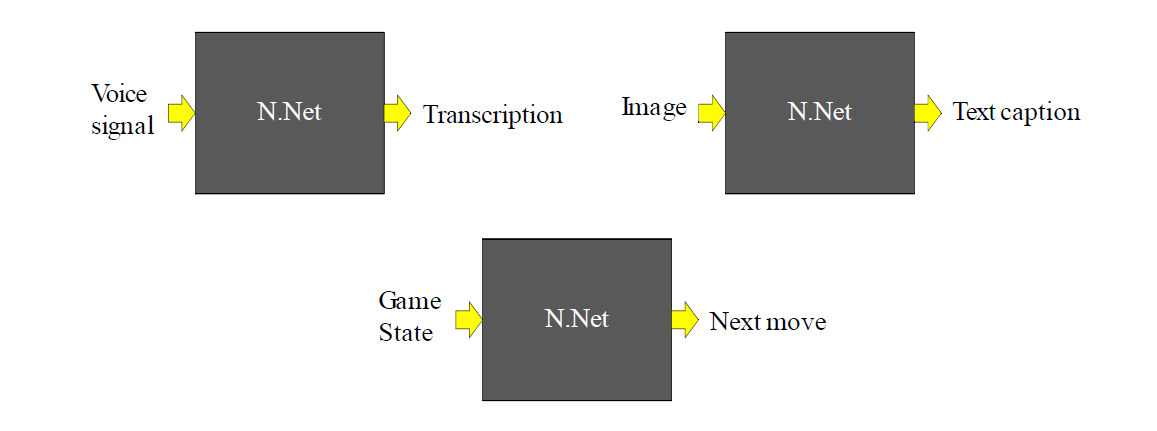
\includegraphics[width=0.9\linewidth]{images/nn_as_function.png}
        \caption{Neural networks act as functions mapping inputs (like voice or images) to outputs (like text or actions).}
    \end{figure}
\end{frame}

\begin{frame}{The Goal: The Formal Problem Setup}
    \framesubtitle{What we have and what we want}
    Based on the previous slides, we can formally define our task:
    \begin{itemize}
        \item \textbf{Given:}
        \begin{itemize}
            \item The \bhighlight{architecture} of the network (e.g., number of layers and neurons).
            \item A set of N \bhighlight{training data} pairs: $(x^{(1)}, y^{(1)}), (x^{(2)}, y^{(2)}), \dots, (x^{(N)}, y^{(N)})$.
        \end{itemize}
        \medskip
        \item \textbf{To Find:}
        \begin{itemize}
            \item The optimal set of \bhighlight{parameters} (weights and biases, denoted collectively as $W$) for our network.
        \end{itemize}
    \end{itemize}
\end{frame}

% --- SLIDE WITH CORRECTION ---
\begin{frame}{The Goal: The Parametric Function and Cost} 
    \framesubtitle{Representing the Network and its Error}
    \begin{itemize}
        \item We consider a neural network as a \bhighlight{parametric function}, $f(x; W)$, where $W$ represents all learnable parameters.
        \item A \bhighlight{loss function}, $\text{loss}(f(x;W), y)$, penalizes the difference between the network's prediction and the desired output for a \emph{single} training example.
        \item The overall \bhighlight{Cost Function} $E(W)$ is the average loss over the \emph{entire} dataset:
        \[
            E(W) = \frac{1}{N} \sum_{n=1}^{N} \text{loss}(f(x^{(n)}; W), y^{(n)})
        \]
    \end{itemize}
\end{frame}

\begin{frame}{The Goal: A Key Requirement}
    \framesubtitle{The Need for Differentiability}
    \begin{itemize}
        \item Our goal is to minimize the cost $E(W)$. To do this with gradient-based methods, the cost function must be \bhighlight{differentiable} with respect to the weights $W$.
        \item This means we must use:
        \begin{itemize}
            \item \textbf{Differentiable Loss Functions:} The way we measure error must be smooth.
            \item \textbf{Continuous Activation Functions:} The functions inside our neurons (like Sigmoid or ReLU) must be differentiable, allowing gradients to flow through the network.
        \end{itemize}
    \end{itemize}
\end{frame}

\begin{frame}{Case Study: Regression}
    \framesubtitle{Output and Loss for Real-Valued Targets}
    \begin{itemize}
        \item For tasks where the desired output is a real number or a vector of real numbers (e.g., predicting a price).
        \item \textbf{Output Layer:} Typically has linear neurons (i.e., no activation function is applied).
        \item \textbf{Loss Function:} The most common choice is the \bhighlight{Squared Error} (or L2 loss):
        \[
            \text{loss}(y, o) = \frac{1}{2} \|y - o\|^2 = \frac{1}{2} \sum_k (y_k - o_k)^2
        \]
    \end{itemize}
    \begin{figure}
        \centering
        % Source: MLP & Back-prop.pdf, Page: 7
        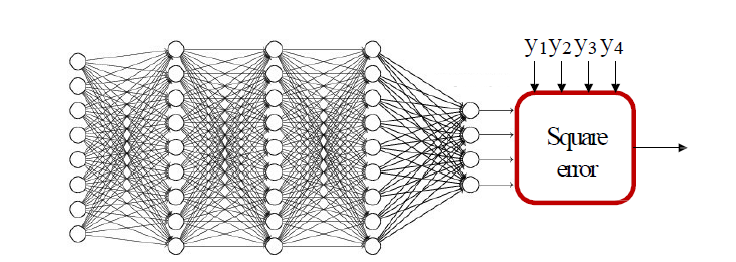
\includegraphics[width=0.8\linewidth]{images/loss_regression.png}
    \end{figure}
\end{frame}

\begin{frame}{Case Study: Binary Classification}
    \framesubtitle{Output and Loss for Two-Class Problems}
    \begin{itemize}
        \item For tasks with two classes (e.g., Cat vs. Dog), where the target $y$ is either 0 or 1.
        \item \textbf{Output Layer:} A single neuron with a \bhighlight{Sigmoid} activation function. This squashes the output to a range of (0, 1), which we can interpret as a probability $P(Y=1|x)$.
        \item \textbf{Loss Function:} \bhighlight{Binary Cross-Entropy} is the standard choice:
        \[
            \text{loss}(y, o) = -y \log(o) - (1 - y) \log(1 - o)
        \]
    \end{itemize}
    \begin{figure}
        \centering
        % Source: MLP & Back-prop.pdf, Page: 11
        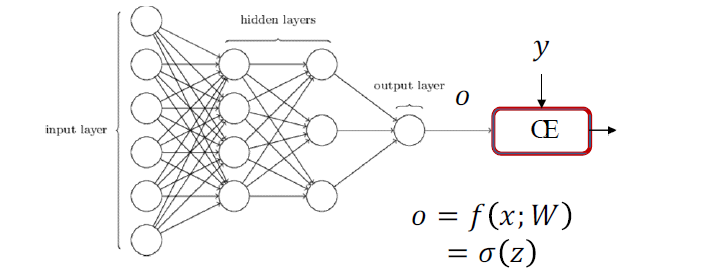
\includegraphics[width=0.6\linewidth]{images/loss_binary_ce.png}
    \end{figure}
\end{frame}

\begin{frame}{Case Study: Multi-Class Classification}
    \framesubtitle{Setup for K > 2 Classes}
    \begin{itemize}
        \item For tasks with multiple classes (e.g., MNIST digits 0-9).
        \item \textbf{Target Representation:} The desired output $y$ is represented as a \bhighlight{one-hot vector}. For example, for class 3 out of 5, $y = [0, 0, 1, 0, 0]^T$.
        \item \textbf{Output Layer:} Must have K neurons, one for each class.
        \item To ensure the outputs are probabilities that sum to 1, we need a special activation function.
    \end{itemize}
\end{frame}

\begin{frame}{Case Study: Multi-Class Classification}
    \framesubtitle{The Softmax Activation}
    \begin{itemize}
        \item The \bhighlight{Softmax} function is used as the activation for the output layer in multi-class problems.
        \item It takes a vector of raw scores (logits) $z$ and transforms it into a probability distribution $o$:
        \[
            o_i = \text{softmax}(z)_i = \frac{\exp(z_i)}{\sum_{j=1}^{K} \exp(z_j)}
        \]
        \item Each output $o_i$ is between 0 and 1, and all outputs sum to 1, making them valid probabilities.
    \end{itemize}
    \begin{figure}
        \centering
        % Source: MLP & Back-prop.pdf, Page: 13
        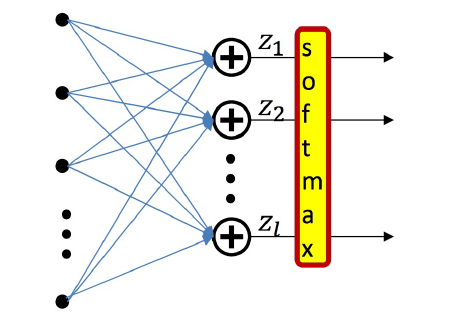
\includegraphics[width=0.5\linewidth]{images/softmax_layer.png}
        \caption{The softmax activation is applied to the final layer.}
    \end{figure}
\end{frame}

\begin{frame}{Case Study: Multi-Class Classification}
    \framesubtitle{Cross-Entropy Loss}
    \begin{itemize}
        \item \textbf{Loss Function:} For multi-class classification, we use the \bhighlight{Cross-Entropy} loss.
        \[
            \text{loss}(y, o) = -\sum_{i=1}^{K} y_i \log(o_i)
        \]
        \item Since $y$ is a one-hot vector, only one term in the sum is non-zero. If the true class is $c$, the formula simplifies to:
        \[
            \text{loss}(y, o) = - \log(o_c)
        \]
        \item This means we are trying to maximize the log-probability of the correct class.
    \end{itemize}
    \begin{figure}
        \centering
        % Source: MLP & Back-prop.pdf, Page: 15
        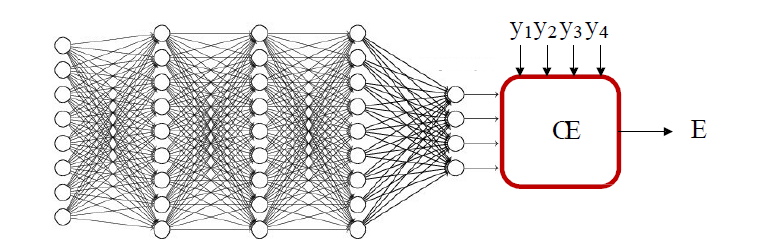
\includegraphics[width=0.8\linewidth]{images/loss_multiclass_ce.png}
    \end{figure}
\end{frame}